\documentclass[tikz,border=8pt]{standalone}
\usepackage{tikz}
\usetikzlibrary{positioning,arrows.meta,shapes.geometric,fit,backgrounds,calc}
\usepackage{fontspec}
\setmainfont{Times New Roman}

\begin{document}
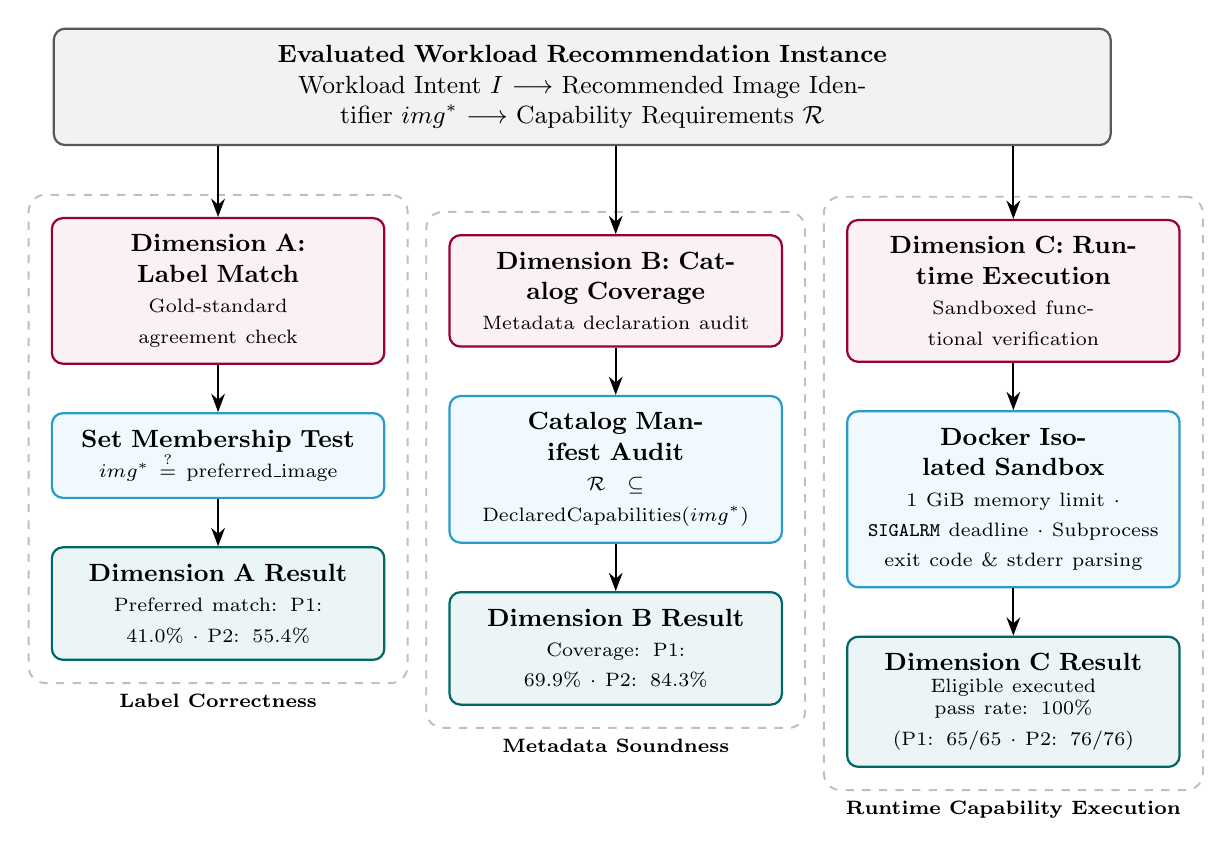
\begin{tikzpicture}[
    font=\small,
    >=Stealth,
    node distance=1.1cm and 0.9cm,
    box/.style={
        draw=blue!70!black,
        fill=blue!5,
        rounded corners=4pt,
        align=center,
        line width=0.8pt,
        inner sep=6pt,
        minimum height=0.9cm
    },
    tier/.style={
        box,
        draw=purple!80!black,
        fill=purple!6,
        text width=3.8cm
    },
    proc/.style={
        box,
        draw=cyan!80!black,
        fill=cyan!6,
        text width=3.8cm
    },
    outbox/.style={
        box,
        draw=teal!80!black,
        fill=teal!8,
        text width=3.8cm
    },
    failbox/.style={
        box,
        draw=red!80!black,
        fill=red!8,
        text width=3.8cm
    },
    group/.style={
        draw=gray!50,
        dashed,
        rounded corners=6pt,
        line width=0.7pt,
        inner sep=8pt
    }
]

% Input Candidate Node
\node[box, fill=gray!10, draw=gray!70!black, text width=13cm] (req) {
    \textbf{Evaluated Workload Recommendation Instance}\\
    Workload Intent $I$ $\longrightarrow$ Recommended Image Identifier $img^*$ $\longrightarrow$ Capability Requirements $\mathcal{R}$
};

% Tier A: Label Match
\node[tier, below=0.9cm of req.south west, xshift=2.1cm] (tier_a) {
    \textbf{Dimension A: Label Match}\\
    \scriptsize Gold-standard agreement check
};
\node[proc, below=0.6cm of tier_a] (proc_a) {
    \textbf{Set Membership Test}\\
    \scriptsize $img^* \stackrel{?}{=} \mathrm{preferred\_image}$
};
\node[outbox, below=0.6cm of proc_a] (out_a) {
    \textbf{Dimension A Result}\\
    \scriptsize Preferred match: P1: 41.0\% $\cdot$ P2: 55.4\%
};

% Tier B: Catalog Capability
\node[tier, right=0.8cm of tier_a] (tier_b) {
    \textbf{Dimension B: Catalog Coverage}\\
    \scriptsize Metadata declaration audit
};
\node[proc, below=0.6cm of tier_b] (proc_b) {
    \textbf{Catalog Manifest Audit}\\
    \scriptsize $\mathcal{R} \subseteq \mathrm{DeclaredCapabilities}(img^*)$
};
\node[outbox, below=0.6cm of proc_b] (out_b) {
    \textbf{Dimension B Result}\\
    \scriptsize Coverage: P1: 69.9\% $\cdot$ P2: 84.3\%
};

% Tier C: Runtime Execution Probe
\node[tier, right=0.8cm of tier_b] (tier_c) {
    \textbf{Dimension C: Runtime Execution}\\
    \scriptsize Sandboxed functional verification
};
\node[proc, below=0.6cm of tier_c] (proc_c) {
    \textbf{Docker Isolated Sandbox}\\
    \scriptsize 1 GiB memory limit $\cdot$ \texttt{SIGALRM} deadline $\cdot$ Subprocess exit code \& stderr parsing
};
\node[outbox, below=0.6cm of proc_c] (out_c) {
    \textbf{Dimension C Result}\\
    \scriptsize Eligible executed pass rate: 100\%\\(P1: 65/65 $\cdot$ P2: 76/76)
};

% Connections
\draw[->, line width=0.8pt] (req.south -| tier_a.north) -- (tier_a.north);
\draw[->, line width=0.8pt] (req.south -| tier_b.north) -- (tier_b.north);
\draw[->, line width=0.8pt] (req.south -| tier_c.north) -- (tier_c.north);

\draw[->, line width=0.8pt] (tier_a) -- (proc_a);
\draw[->, line width=0.8pt] (proc_a) -- (out_a);

\draw[->, line width=0.8pt] (tier_b) -- (proc_b);
\draw[->, line width=0.8pt] (proc_b) -- (out_b);

\draw[->, line width=0.8pt] (tier_c) -- (proc_c);
\draw[->, line width=0.8pt] (proc_c) -- (out_c);

% Group backgrounds
\begin{scope}[on background layer]
    \node[group, fit=(tier_a)(out_a), label=below:{\scriptsize \textbf{Label Correctness}}] {};
    \node[group, fit=(tier_b)(out_b), label=below:{\scriptsize \textbf{Metadata Soundness}}] {};
    \node[group, fit=(tier_c)(out_c), label=below:{\scriptsize \textbf{Runtime Capability Execution}}] {};
\end{scope}

\end{tikzpicture}
\end{document}
